\documentclass{article}

\usepackage{graphicx}
\usepackage{tikz}
\usepackage{tikzsymbols}
\usetikzlibrary{calc,patterns,shapes.geometric}
\pagestyle{empty}
\usepackage[margin=0pt]{geometry}
\geometry{papersize={14in,12in}}

\def\centerarc[#1](#2)(#3:#4:#5){\draw[#1] ($(#2)+({#5*cos(#3)},{#5*sin(#3)})$) arc (#3:#4:#5);}

\begin{document}
	\begin{figure}
		\centering
		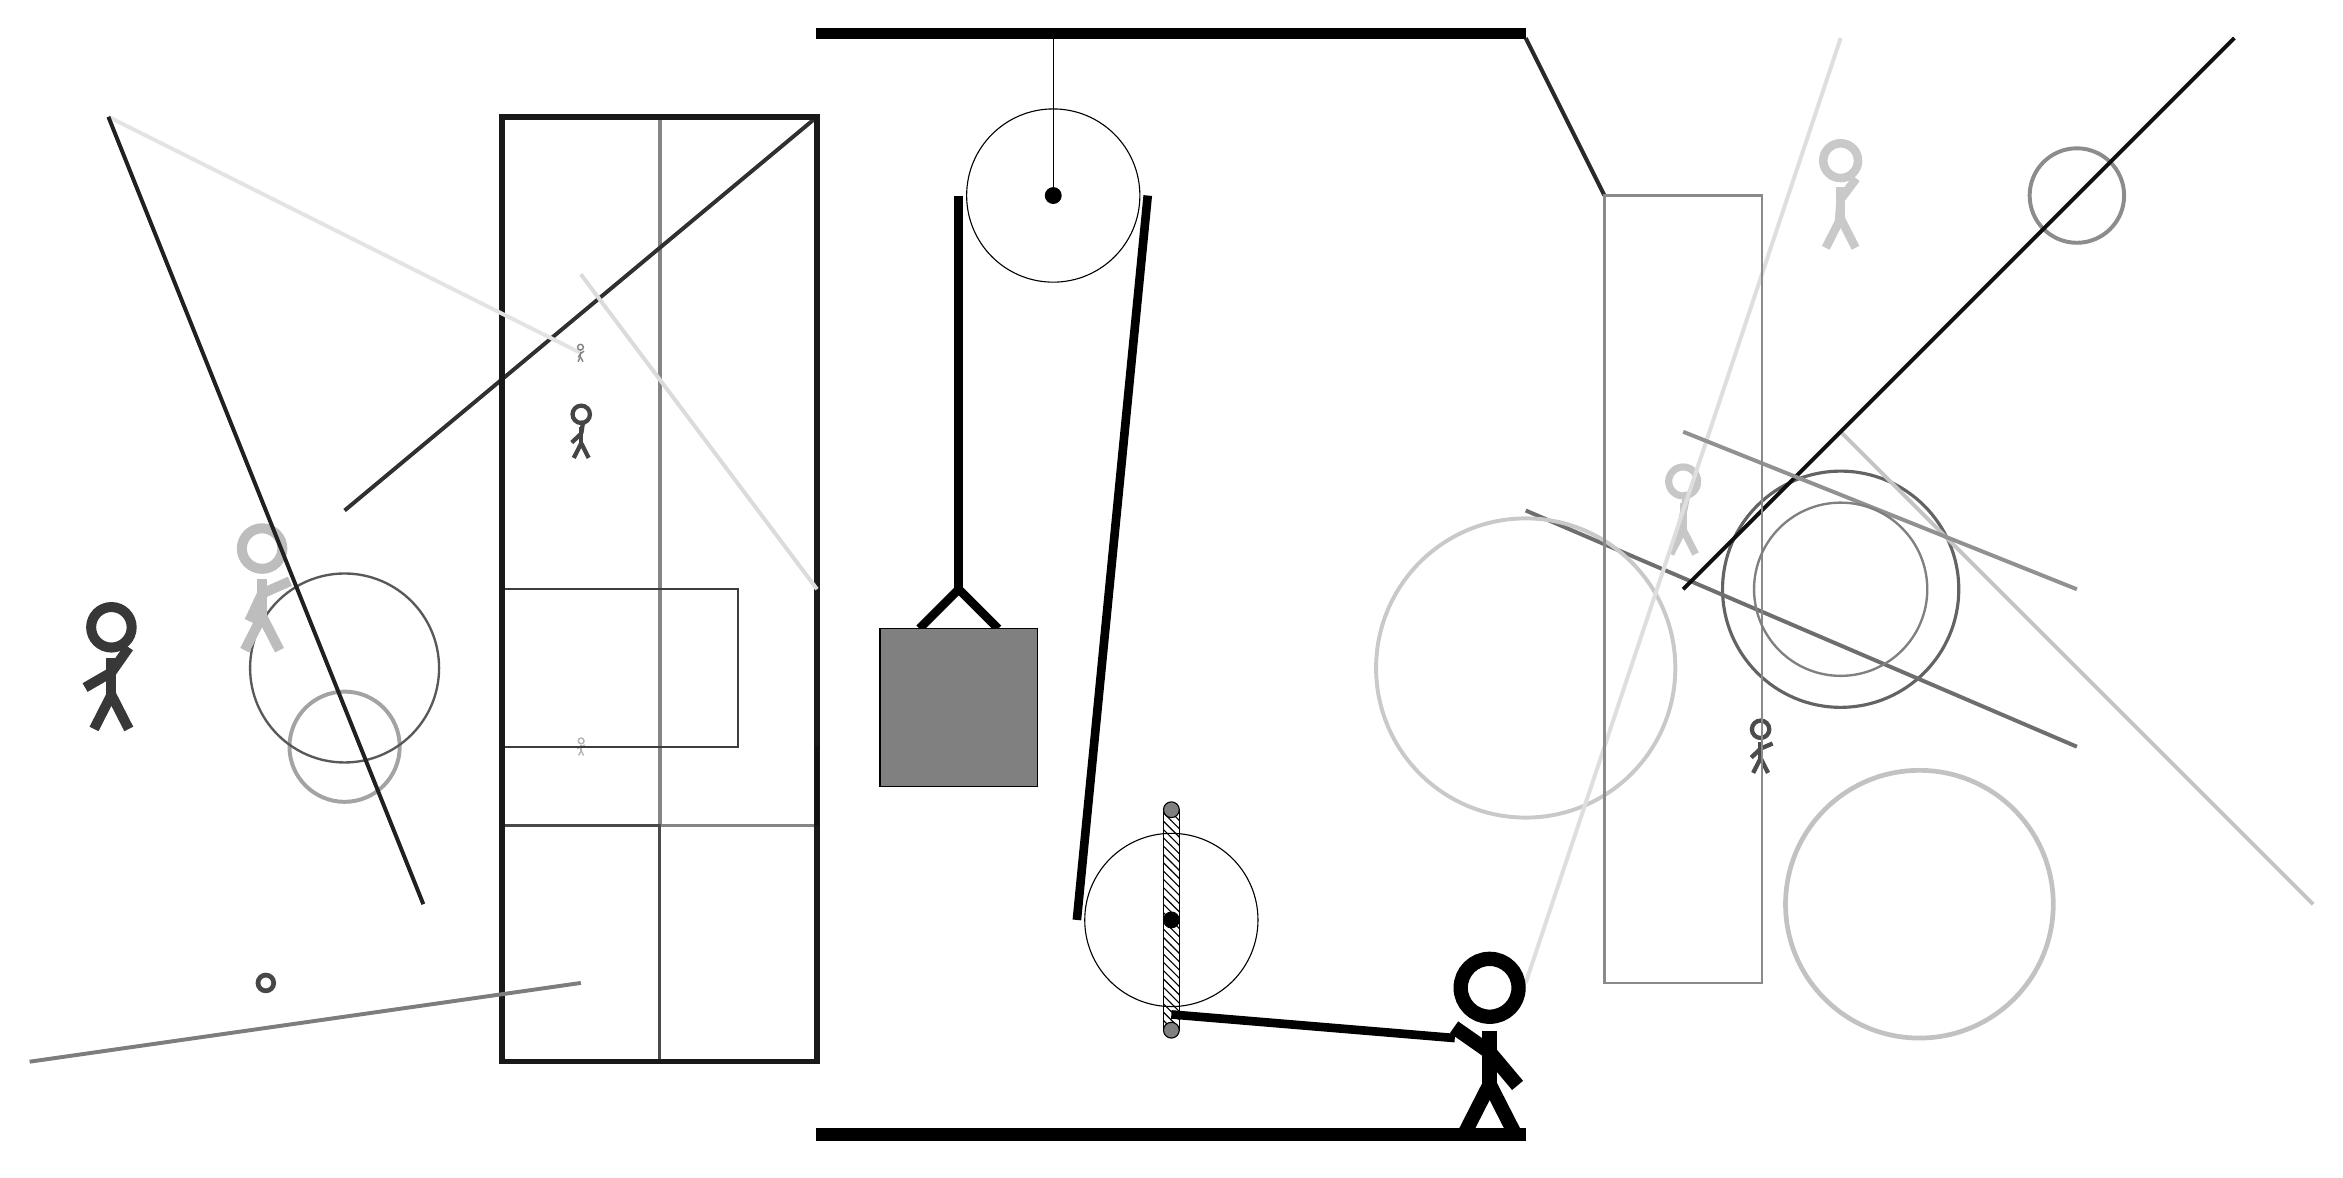
\begin{tikzpicture}
			%%%%% START %%%%%
			
			\draw[fill=black] (-2, 14) rectangle (7, 14.125);
			
			\draw (1, 12) circle (1.1);
			\draw[fill=black] (1, 12) circle (0.1);
			\draw (1, 14) -- (1, 12);
			
			\draw[fill=white](2.5, 2.8) circle (1.1);
			\draw[fill=black] (2.5, 2.8) circle (0.1);
			\draw[pattern=north west lines, pattern color=black] (2.4, 4.2) rectangle (2.6, 1.4);
			\draw[fill=black!50] (2.5, 4.2) circle (0.1);
			\draw[fill=black!50] (2.5, 1.4) circle (0.1);
			
			\draw[line width=1.1mm] (-0.7, 6.5) -- (-0.2, 7.0) -- (0.3, 6.5);
			\draw[fill=black!50] (-1.2, 6.5) rectangle (0.8, 4.5);
			
			\draw[line width=0.5mm, color=black!48] (-2, 13) rectangle (-4, 4);
			
			\node[line width=0.3mm, color=black!29] at (-5, 5) {\Strichmaxerl[1][11][34]};
			\node[line width=0.2mm, color=black!70] at (10, 5) {\Strichmaxerl[3][44][23]};
			\draw[line width=0.3mm, color=black!76] (-3, 7) rectangle (-6, 5);
			\draw[line width=0.3mm, color=black!71] (-4, 1) rectangle (-6, 4);
			\draw [line width=0.4mm, color=black!61](11, 7) circle (1.5);
			\draw[line width=0.5mm, color=black!57](7, 8) -- (14, 5);
			\draw [line width=0.6mm, color=black!72](-9, 2) circle (0.1);
			\draw [line width=0.5mm, color=black!21](7, 6) circle (1.9);
			
			\draw [line width=0.5mm, color=black!36](-8, 5) circle (0.7);
			\draw [line width=0.6mm, color=black!24](12, 3) circle (1.7);
			\draw[line width=0.5mm, color=black!23](11, 9) -- (17, 3);
			\node[line width=0.5mm, color=black!73] at (-5, 9) {\Strichmaxerl[3][43][81]};
			
			\draw[line width=0.5mm, color=black!81](-2, 13) -- (-8, 8);
			\draw[line width=0.5mm, color=black!84](7, 14) -- (8, 12);
			\node[line width=0.7mm, color=black!22] at (9, 8) {\Strichmaxerl[5][79][79]};
			
			\draw [line width=0.3mm, color=black!65](-8, 6) circle (1.2);
			\node[line width=0.2mm, color=black!26] at (-9, 7) {\Strichmaxerl[7][65][24]};
			\node[line width=0.3mm, color=black!21] at (11, 12) {\Strichmaxerl[6][86][53]};
			\draw[line width=0.7mm, color=black!90] (-2, 13) rectangle (-6, 1);
			\draw [line width=0.5mm, color=black!45](14, 12) circle (0.6);
			
			\draw[line width=0.5mm, color=black!11](-5, 10) -- (-11, 13);
			
			\draw[line width=0.5mm, color=black!94](9, 7) -- (16, 14);
			\node[line width=0.3mm, color=black!49] at (-5, 10) {\Strichmaxerl[1][59][35]};
			\draw[line width=0.5mm, color=black!13](11, 14) -- (7, 2);
			\draw[line width=0.5mm, color=black!14](-5, 11) -- (-2, 7);
			\draw[line width=0.5mm, color=black!43](9, 9) -- (14, 7);
			\draw[line width=0.4mm, color=black!93] (-2, 4) rectangle (-2, 5);
			\node[line width=0.5mm, color=black!78] at (-11, 6) {\Strichmaxerl[7][30][55]};
			
			\draw[line width=0.3mm, color=black!46] (8, 12) rectangle (10, 2);
			\draw[line width=0.5mm, color=black!87](-7, 3) -- (-11, 13);
			
			\draw [line width=0.3mm, color=black!50](11, 7) circle (1.1);
			\draw[line width=0.5mm, color=black!51](-5, 2) -- (-12, 1);
			
			
			\draw[line width=1.1mm] (-0.2, 12) -- (-0.2, 7.0);
			\centerarc[line width=1.1mm](1, 12)(0:180:1.2000000000000002);
			\draw[line width=1.1mm](2.2, 12) -- (1.3, 2.8);
			\centerarc[line width=1.1mm](2.5, 2.8)(180:270:1.2000000000000002);
			\draw[line width=1.1mm](2.5, 1.6) -- (6.1, 1.3);
			
			\node at (6.5, 1.2) {\Strichmaxerl[10][-35][-50]};
			
			\draw[fill=black] (-2, 0) rectangle (7, 0.15);
			
			%%%%% END %%%%%
		\end{tikzpicture}
	\end{figure}	
\end{document}